\documentclass[a4paper, oneside]{book}
\usepackage[italian]{babel}
\usepackage[utf8]{inputenc}
\usepackage[a4paper,top=2.5cm,bottom=2.5cm,left=2cm,right=2cm]{geometry}
\usepackage{amssymb}
\usepackage{amsthm}
\usepackage{graphics}
\usepackage{amsfonts}
\usepackage{amsmath}
\usepackage{amstext}
\usepackage{engrec}
\usepackage{rotating}
\usepackage[safe,extra]{tipa}
\usepackage{multirow}
\usepackage{hyperref}
\usepackage{enumerate}
\usepackage{braket}
\usepackage{marginnote}
\usepackage{pgfplots}
\usepackage{cancel}
\usepackage{polynom}
\usepackage{booktabs}
\usepackage{enumitem}
\usepackage{algorithm}
\usepackage{algpseudocode}
\usepackage{framed}
\usepackage{pdfpages}
\usepackage{pgfplots}
\usepackage{fancyhdr}
\usepackage{caption}
\usepackage{subcaption}
\usepackage{setspace}
\usepackage{hyperref}
\pagestyle{fancy}
\fancyhead[L,RO]{\slshape \rightmark}
\fancyfoot[C]{\thepage}

\title{Data and Computational Biology}
\author{Tommaso Ferrario (\href{https://github.com/TommasoFerrario18}{@TommasoFerrario18})}
\date{Ottobre 2024}

\pgfplotsset{compat=1.13}

\begin{document}

\maketitle
\newtheorem{teorema}{Teorema}
\newtheorem{dimostrazione}{Dimostrazione}
\newtheorem{definition}{Definition}
\newtheorem{esempio}{Esempio}
\newtheorem{osservazione}{Osservazione}
\newtheorem{note}{Note}
\newtheorem{corollario}{Corollario}
\tableofcontents
\renewcommand{\chaptermark}[1]{
    \markboth{\chaptername
        \ \thechapter.\ #1}{}}
\renewcommand{\sectionmark}[1]{\markright{\thesection.\ #1}}

\chapter{Introduction}
In this course, we will study the principles of modeling and analysis biology
data using simulation and AI models.

In the field of biology, the scale size varies from the organism like tree passing
through tissues and arriving at the cellular level. So we are considering elements
with the size that varies from meters to micrometers.

In particular, we can distinguish two main groups of organisms: bacteria and eukaryotes.

All this organisms have in common that all have DNA as genetic material. The DNA
is a molecule that contains the information necessary to build and maintain an
organism.

We can describe the DNA as a sequence of nucleotides. The nucleotides are the
building blocks of DNA. The DNA is a double helix structure, and the nucleotides
are paired in a specific way. The nucleotides are \textit{adenine}, \textit{thymine},
\textit{cytosine}, and \textit{guanine}.

This nucleotides are paired in the following way: \textit{adenine} with \textit{thymine}
and \textit{cytosine} with \textit{guanine}. This help us to save up space because
they are always complementary.

A \textbf{gene} is a sequence of nucleotides that contains the information to
create a protein. While a \textbf{genome} is the complete set of genes of an organism.

\begin{figure}[!ht]
    \centering
    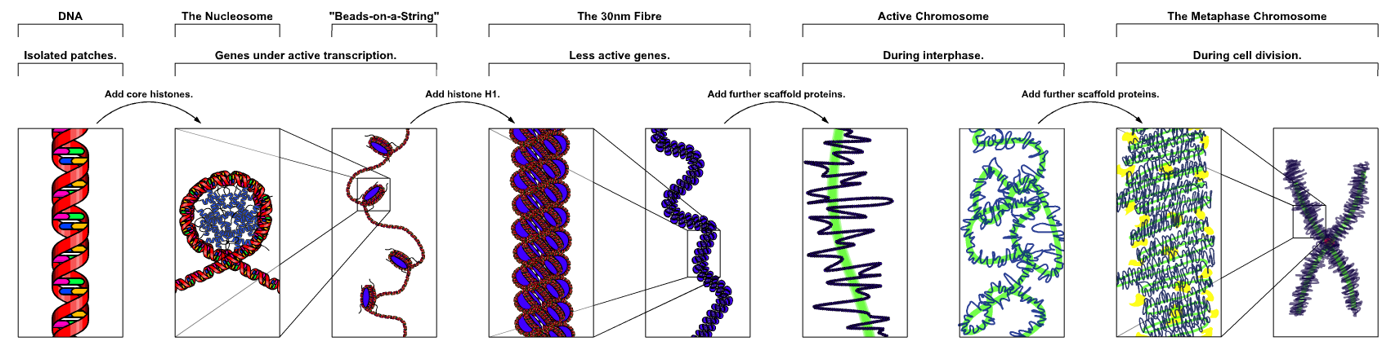
\includegraphics[width=\textwidth]{img/DNA.png}
    \caption{DNA structure}
    \label{fig:dna}
\end{figure}

A \textbf{genomic arm} refers to a large segment of a chromosome, typically
spanning several megabases (Mb) in size.

Starting from DNA we can create \textbf{RNA} through a process called \textbf{transcription}.
The RNA is a molecule that is used to create proteins. The proteins are the
building blocks of the cells. The process of creating proteins from RNA is called
\textbf{translation}.

The RNA transport information from nucleus, in other words, the DNA, to the
cytoplasm of a cell, where it mediates the process of translation to create proteins.

Once the information has passed into the protein it cannot get out again. The
transfer information from nucleic acid to nucleic acid, or from nucleic acid to
protein may be possible, but the transfer information from protein to protein,
or from protein to nucleic acid is impossible.
\section*{The Repressillator example}
A useful example to use as a base for the course is the repressillator. This is a
simple model of a genetic network that is able to oscillate. In particular, it is
compose of three proteins, $LacI$, $TetR$ and $\lambda CI$, that repress each other.

The structure of the repressillator is shown in Figure \ref{fig:repressillator}.
We can observe a circular structure, where each protein represses the next one in
the circle. This is a simple model of a genetic network that is able to oscillate.
More specifically, the LacI protein inhibits transcription of the second repressor
gene, TetR, which in turn inhibits the third repressor gene, $\lambda$ CI, which
in turn inhibits the first repressor gene, LacI.
\begin{figure}[!ht]
    \centering
    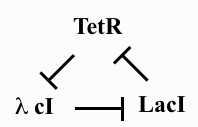
\includegraphics[width=0.5\textwidth]{img/repressillator.png}
    \caption{Structure of the repressillator.}
    \label{fig:repressillator}
\end{figure}

To implements this model, two \textbf{plasmids} are used. The plasmids are small
circular DNA molecules that are separate from the chromosomal DNA and can replicate
independently. The first plasmid codifies for the three proteins, while the second
plasmid serve as reporter of the system (GFP).

This system can be modeled using a set six of ordinary differential equations,
two for each protein. The general form of the equations is:
\begin{itemize}
    \item One equation for the variation of mRNA:
          \begin{equation}
              \frac{dM_i}{dt} = -m_i + \frac{\alpha}{1 + p_j^n} + \alpha_0
          \end{equation}
    \item One for representing the variation of the protein:
          \begin{equation}
              \frac{dP_i}{dt} = \beta (m_i - p_i)
          \end{equation}
\end{itemize}
where:
\begin{itemize}
    \item $\alpha$ is the proteins/cell from non repressed promoter.
    \item $\alpha_0$ is the proteins/cell from repressed promoter.
    \item $\beta$ protein mRNA decay velocity.
    \item $n$ Hill's coperativity coefficient.
\end{itemize}
\section{System, Biotech measures and Analysis}
During this course we want to measure two things:
\begin{itemize}
    \item \textbf{Gene expression}.
    \item \textbf{Gene alteration} also known as \textbf{mutation}.
\end{itemize}

The technology to obtain the information has evolved over time. In particular,
we have used \textit{microarrays} to measure gene expression, and now we use
\textit{next-generation sequencing} (NGS) for almost everything.

To collect data about gene expression, we can use \textbf{differential gene
    expression} (DGE). After using this approach, we can apply statistical
operation such as clustering or enrichment with genome ontology (GO).

With the enrichment phases we want to associate representative terms to the
clustering we have obtained. This operation is done in order to point out the
most important terms that are associated with the clustering.

\textbf{Gene ontology} is a controlled vocabulary that is use to describe gene.
It is divided in three categories:
\begin{itemize}
    \item \textbf{Biological process}: the biological objective to which the gene
          contributes.
    \item \textbf{Molecular function}: the biochemical activity of the gene product.
    \item \textbf{Cellular component}: the location of the gene product.
\end{itemize}
This information are express using a directed acyclic graph (DAG) where the main
type of association are \textbf{is a} and \textbf{part of}.
\subsection{Next-Generation Sequencing}
\textbf{Next-generation sequencing} (NGS) is a high-throughput methodology that
enables rapid sequencing of the base pairs in DNA or RNA samples.

The \textbf{sequencing} operation consists into fragmenting and extraction of
the DNA, then the DNA is sequenced and the \textbf{reads} are obtained. The reads
are short DNA fragments that are obtained from the sequencing process.

As computer scientists, we are interested in the dry-lab analysis which consists
in the \textbf{assembly} the \textit{reads} into a \textbf{Contigs}. Also, they
need to solve problem related to reads storage and allignments.

Talking about NGS, we can distinguish different approaches:
\begin{itemize}
    \item \textbf{Whole-genome sequencing} (WGS): the process of determining the
          complete DNA sequence of an organism's genome at a single time. This
          can be \textit{de novo} which mean that we don't have any reference
          genome.
    \item \textbf{Exome sequencing}: the process of capturing and sequencing the
          coding region of the genome.
    \item \textbf{Targeted sequencing}: the process of capturing and sequencing
          specific regions of the genome.
    \item \textbf{RNA sequencing} (RNA-Seq): the process of determining the
          complete RNA sequence of an organism's genome at a single time.
\end{itemize}

Also, talking about the analysis we can distinguish two types of analysis:
\begin{itemize}
    \item \textbf{Bulk analysis}: in this approach we use a pool of cells to analyze
          the gene expression. In particular, we create a average cell where we
          can study the overall gene expression.
    \item \textbf{Single cell analysis}: in this approach we analyze the gene
          expression of a single cell. This approach is more expensive and complex
          but it allows to study the gene expression of a single cell.
\end{itemize}
\subsection{From Sequencing to Mutational Information}
Thanks to the NGS we can obtain sequence that reveal different aspect of a
biological phenomenon. In this case, we can describe different subtypes of
mutations. Also, using bulk sequencing we can build a phylogeny tree that
describe the evolution of the mutation.
\chapter{Chemistry and Reactions}
\begin{definition}[\textbf{Mixture}]
    In chemistry the forms of matter are called \textbf{mixtures}. Some of them
    are \textbf{homogeneous} and others are \textbf{solution} with a \textbf{solvent}
    and a \textbf{solute}.

    To separate the components of a mixture we can use different methods like
    \textbf{filtration}, \textbf{distillation}, \textbf{chromatography} and
    \textbf{evaporation}.
\end{definition}
\begin{definition}[\textbf{Compound}]
    Certain substances are not separable by simple physical methods. These are
    called \textbf{compounds} and are formed by the union of two or more elements.
\end{definition}
\begin{definition}[\textbf{Reactions}]
    Pure substances cannot be further separated by means of physical interventions,
    but can be modified by means of (bio)chemical reactions.

    A reaction involves a certain number of reactants, yielding a number of products.
    \begin{equation}
        R_1 \bigoplus R_2 \bigoplus \ldots \bigoplus R_n \rightarrow P_1
        \bigoplus P_2 \bigoplus \ldots \bigoplus P_m
    \end{equation}

    As we all know, there are bits of matter that cannot be modified at the
    chemical level. These are called \textbf{elements}.
\end{definition}
\begin{definition}[\textbf{Atoms}]
    Atoms are composed by nuclei (protons and neutrons) and electrons on (quantized)
    orbits. Every orbit can contain up to 8 electrons (except for the first,
    which can hold only 2) this fact is known as the octect rule.

    The most external orbit is, except for the “noble gases”, incomplete; the
    number of electrons that occupy them determine the atom valence.
\end{definition}

The configuration of the external orbits of atoms, allows them to bind together
in compounds. Molecule structure depends on the organization of the electron
sharing in the most external orbits.

Atoms with valence up to 4 tend to be electron donors to atoms with a valence
from 5 to 7; atoms are therefore grouped in donors and receptors. Receptors atoms
are said to have an electronegative tendency.

There are several ways atoms bind to each other, the most common are:
\begin{itemize}
    \item \textbf{Ionic bindings} happen between atoms with very different valence.
    \item \textbf{Covalent bindings} happen between atoms of similar valence.
\end{itemize}

Molecules have a polarity, depending on the electronegativity of each participant
atom and their spatial configuration. Polar molecules tend to attract each other,
while non-polar molecules are relatively.

The forces that create bonds between atoms are also responsible of the attraction
between atoms and molecules. An intermediate attraction force is that resulting
from \textbf{hydrogen bonds} which keep together the DNA double helix.
\section{Reactions and Metabolism}
Biochemical reactions modify properties of various compounds and we can classify
them in two main categories:
\begin{itemize}
    \item \textbf{Reversible reactions} are those that can be reversed by changing
          the conditions of the system. They can be analyze at the equilibrium.
    \item \textbf{Irreversible reactions} are those that cannot be reversed.
\end{itemize}
The quantitative ratio among compounds in a reaction is called the reaction
\textbf{stoichiometry}.
The translation of stoichiometric ratios into physical quantities and vice-versa
requires the introduction of new units. So, chemists have defined the \textbf{mole}
as the quantity of substances comprising about $6.022 \times 10^{23}$ molecules.

This analysis is performed by looking at concentrations of a substance, measured
in mole/liter; this dimension is called the molarity of a solution.

Every reaction has its own reaction rate also called velocity. Given a reaction,
when the concentration of a reactant is very low, or the reaction rate is very
slow, then the reaction is said to be kinetically impaired.

A reaction can happen only when a positive $\Delta G$ is present and that is
enough to exceed the so-called activation barrier; such amount of energy is known
as activation energy.

Energy contained in ATP phosphate bonds is sufficient for the activation of
several biochemical reaction. This energy is however not enough to endanger several
of the other bond types that are present in an organism.

The metabolism is the activity that allows an organism to survive. This process
is mostly carried out in the cytoplasm of the cells and we can divide it in two
main categories:
\begin{itemize}
    \item \textbf{Catabolism} is the set of reactions that decompose various
          complexes, mostly acquired from the environment.
    \item \textbf{Anabolism} is the set of reactions that synthesize complexes.
\end{itemize}

Many of the basic reactions are shared, without much variation, by most living
organisms this is known as core metabolism. The metabolism that is specialized
for a class of organisms is dubbed secondary metabolism.

A very important process is the one that allows an organism to “load” ADP molecules
with a phosphate group, thus generating ATP. To obtain this result, organisms use
chains of reactions, called \textbf{metabolic pathways}.

Several of these reactions have a rather high activation energy or a quite slow
reaction rate. To speed up such reactions, organisms use the catalysis machinery.
A catalyzer speeds up a reaction or lowers its activation energy without being
consumed. Catalyzers are called enzymes, acting on substrates.
\section{Mathematical Modeling of Reactions}
Much of Computational Biology is \textbf{modeling reaction networks} which can be
subdivided in two main categories:
\begin{itemize}
    \item \textbf{Metabolic networks} are the set of reactions that take place
          in a cell. These reactions are mostly catalyzed by enzymes.
    \item \textbf{Regulatory networks} are the set of reactions that regulate
          the activity of the metabolic networks.
\end{itemize}
\subsection{Law of Mass-Action}
Collision between two chemical compounds $A$ and $B$ happen with a rate $k$ and
produce a compound $C$.
\begin{equation*}
    A + B \xrightarrow{k} C
\end{equation*}

We can rewrite the previous equation as:
\begin{equation}
    \frac{\delta [C]}{\delta t} = k [A][B]
\end{equation}
where with $[A]$ we denote the concentration of compound $A$. As said before,
we have also reaction that can be reversed, so we can write:
\begin{equation}
    A + B \mathrel{\mathop{\rightleftarrows}^{\mathrm{k_1}}_{\mathrm{k_2}}} C
\end{equation}
and the rate of the reaction is:
\begin{equation}
    \frac{\delta [A]}{\delta t} = k_2 [C] - k_1 [A][B]
\end{equation}
When a system is at equilibrium, the concentration don't change, therefore the
following condition holds:
\begin{equation}
    \frac{k_1}{k_2} = K_{eq} = \frac{[A]_{eq} [B]_{eq}}{[C]_{eq}}
\end{equation}
where $K_{eq}$ is the equilibrium constant of the reaction. If $K_{eq}$ is small,
then this is an indication that, at equilibrium, the concentration of $A$ and $B$
are effectively combined to form $C$.

Enzymatic reactions, which are non elementary reactions, can be modeled by the
Michaelis-Menten equation:
\begin{equation}
    S + E \mathrel{\mathop{\rightleftarrows}^{\mathrm{k_1}}_{\mathrm{k_2}}} catalysis \xrightarrow{k_3} P + E
\end{equation}
where $S$ is the substrate, $E$ is the enzyme, $P$ is the product and catalysis
and $C$ is the intermediate product.

Let's now consider the total enzyme concentration to be $[E]_0 = [E] + [C]$ and
also that all the reaction rate are constant. We can define the velocity at which
we increase the product concentration is:
\begin{equation}
    \frac{\delta [P]}{\delta t} = k_3 [C] \approx [E][S]
\end{equation}
so we can say that the velocity is proportional to the concentration of $[E]$ and
$[S]$.

The Michaelis-Menten system can be analytically solved by an equilibrium
approximation where we assume that the substrate $S$ and the complex $C$ are in
instantaneous equilibrium. This assumption allows us to write the following:
\begin{equation}
    k_1[S][E] = k_2[C] + k_3[C]
\end{equation}
Since $[E]_0 = [C] + [E]$, we can rewrite the previous equation as:
\begin{equation}
    [S][E]_0 - [S][C] = [C]\left( \frac{k_1 - k_3}{k_2}\right)
\end{equation}
We now introduce the Michaelis constant $K_M = \frac{k_2 + k_3}{k_1}$ which is
the combination of the rate constants of the reaction. We can rewrite the previous
equation as:
\begin{equation}
    [C] = \frac{[S][E]_0}{K_M + [S]}
\end{equation}
The velocity of the creation of $P$ is then:
\begin{equation}
    V = \frac{\delta [P]}{\delta t} = k_3[C]
\end{equation}
At $V_{max}$ we have that all the enzyme $E_0$ must be bound in the complex $C$,
this means that:
\begin{equation}
    V_{max} = k_3[E]_0
\end{equation}

If we now put everything together, we can write the Michaelis-Menten equation as:
\begin{equation}
    V = \frac{V_{max}[S]}{K_M + [S]}
\end{equation}
We can say that the Michaelis-Menten constant is a concentration ($\approx [S]$)
at which the velocity is half of $V_{max}$. In formula:
\begin{equation}
    V = \frac{V_{max}[S]}{K_M + [S]} = \frac{V_{max}}{2}
\end{equation}
\chapter{Computational Modeling}
\section{Deterministic Models}
We start by considering a deterministic model, which is a system of ordinary
differential equations (ODEs) that describe the time evolution of the
concentrations of the species in the system.

The main issue of deterministic models is \textbf{time}, which is represented
as a discrete variable.

The standard tool use to model deterministic models is the \textbf{ordinary
    differential equations} (ODEs). The ODEs are a set of equations that describe
the time evolution of the concentrations of the species in the system.

A different approach is to use \textbf{discrete event simulation} (DES), which
are a queue of events generated by a sources and processed by components. In this
representation, time is usually a derived notion, for example observing the
sequence of events.

\subsection{Stem Cell Differentiation}
The first model we consider is the stem cell differentiation model. The
\textbf{stem cell} differentiate into \textbf{progenitor cells}, which in turn
differentiate into \textbf{regular cells}.

The division or proliferation of stem cell can be:
\begin{itemize}
    \item \textbf{Symmetric}: the stem cell divides into two stem cells.
    \item \textbf{Asymmetric}: the stem cell divides into one stem cell and one regular cell.
    \item \textbf{Envirormentally Asymmetric}: the stem cell divides into one
          stem cell and one progenitor cell.
\end{itemize}

A first simple model of stem cell can be represented by a finite state machine
describe in Figure \ref{fig:stem_cell_fsm}.

\begin{figure}[!ht]
    \centering
    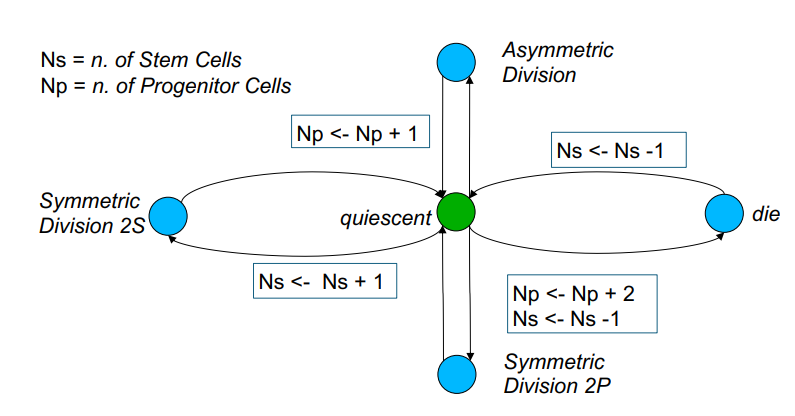
\includegraphics[width=.7\textwidth]{img/stemcellsFSA.png}
    \caption{Stem Cell Finite State Machine}
    \label{fig:stem_cell_fsm}
\end{figure}

In this example we don't consider the time. Time can be model considering an
exponential delay to the transition. Moreover, we can associate a different
probability to each transition, so we have a transition system (Markov Chain).
\section{Implementing a simulator}
In order to implement a simulator we need to define what means for us to run a
simulation. We can define a simulation as a sequence of events that can be
described by numerically solving a set of ODEs or by tracking the sequence of
events in a DES. This produce a \textbf{trace} of the simulation.

A trace is a sequence of vectors of values, where each vector represents the
state of the system at a given time. The trace can be used to analyze the
behavior of the system.

The engine of a simulator is essentially a loop where is body determines the
type of simulator we are using.
\subsection{Finite State Automata Simulator}
To implement a finite state automata simulator we need to define the following
elements:
\begin{itemize}
    \item \textbf{Specification}: first we need to define a set of finite
          automata, each represented by a matrix.
    \item \textbf{Engine}: check the set of all the enabled transitions from the
          current state and produce the next state.
    \item \textbf{Specification}: sources, computing units and sinks.
    \item \textbf{Trace}: a sequence of states.
\end{itemize}

\chapter{Spatial Simulation}
We want now study some simulation method that involve the spatial 
component. 
\section*{Colonic Crypts}
We will present the different simulation techniques starting from 
a base example regurding the \textbf{colon cancer}.

This type of cancer originates in \textbf{colonic crypts}, where 
there are stem cells that divide to reproduce the \textit{epithelium}.
The cells generated move up from the crypts. During this journey 
they evolve in different types:
\begin{itemize}
    \item absorptive cell
    \item goblet cell
    \item enteroendocrine cell
    \item Paneth cell
\end{itemize}

Also, we are intrested in the evolution of the tumor which can be
describe as follow:
\begin{itemize}
    \item All starts from a normal epithelium.
    \item It can happen that some cells acquire a mutation on APC or 
        $\beta$-catenin genes.
    \item If the mutation remains and the cells start reproducing
        losing the regulation mechanisms. In this situation we have
        an \textit{initial adenoma}.
    \item If the cells mutate the K-RAS gene. In this situation we 
        have an \textit{intermidiate adenoma}.
    \item At this point the cell can recive a mutation on different
        gene (DCC, SMAD4 and SMAD2) bringing the system to a 
        situation of \textit{final adenoma}.
    \item If it also add a mutation on \textbf{p53}, which is a gene 
        that is responsible for the suicde of the cell.
    \item at the end we have the metastasi. 
\end{itemize}
However, there are other types of colon cancer, such as Hereditary Non-Polyposis Colorectal Cancer (HNPCC), which is characterized by a distinct set of genetic mutations.

There are also various mechanisms involved in tumor development, including the Vascular 
Endothelial Growth Factor (VEGF) pathway, which is responsible for angiogenesis, the process 
by which new blood vessels form from pre-existing ones.

\section{Simulation}
In modeling a tumor tissue, different paradigms and levels of abstraction, parameters, and considerations are applied. Besides the model’s implementation itself, it is essential to determine the constraints to consider and the variables to observe.

\subsection{In-Lattice Models}
The key factor distinguishing different models is how the main agents—specifically, the cells—are represented. In in-lattice models, a cell is depicted as a collection of positions on a grid.

\subsubsection{Cellular Potts Model}
A significant in-lattice model is the Cellular Potts Model (CPM), a type of cellular automaton. It was developed to study the Differential Adhesion Hypothesis (DAH), which, in simple terms, suggests that if two cell populations are mixed and adhere to each other, the system will eventually reorganize into layers.

This system is implemented by calculating the total energy of the system (denoted by Potts as $J$), which depends on the adhesion parameters between different types of cells. The system's energy depends on the relative positions of various cells. The system evolves by calculating $J$ step-by-step, and each move is chosen to minimize $J$.

We use a two-dimensional grid, where each square or pixel, identified by coordinates \((i, j)\), is assigned values:
\begin{itemize}
    \item \(\sigma(i,j) =\) id, a function that assigns an id to indicate the cell to which each pixel belongs;
    \item \(\tau(\sigma(i,j)) =\) type, a function that assigns a type to each cell;
\end{itemize}

The total energy of the CPM is associated with the surface area of the cells, represented by the function:
\[
J(\tau, \tau')
\]
which indicates the surface energy per unit of contact between two cells. Energy is lower between pixels belonging to cells of the same type, higher for cells of different types, and zero between pixels of the same cell.

The total energy of the CPM is defined as the sum of the energies calculated for cell surfaces plus a constant multiplied by the energy associated with a cell's area:
\[
H_{Potts} = H_{surface} + \lambda H_{Area}
\]
where \(H_{Potts}\) is a Hamiltonian operator and \(\lambda\) is the rigidity constant of the cytoskeleton, serving as a Lagrange multiplier.

\subsubsection{Wong Model}
This model enables the modeling of motility—the capacity of a living organism, or part of it, to actively and reversibly change its position relative to its environment—for both stem cells and progenitor cells within crypts.

It is a two-dimensional model that includes several constraints, including:
\begin{itemize}
    \item An energy term that keeps stem cells fixed in predefined positions.
    \item Specific rules that model cell growth, division, and apoptosis.
    \item A fundamental model assumption regarding the most significant morphogen considered.
\end{itemize}

The final simulation outcome allows us to observe that:
\begin{itemize}
    \item Differential adhesion regulates cell positioning within the crypt.
    \item Epithelial cells move vertically toward the lumen of the crypt.
    \item Despite relatively few assumptions, the movement is coordinated.
    \item The homeostasis of intestinal epithelial cells is maintained in the model.
\end{itemize}

It is worth noting that the simulation remains relatively simple with few assumptions.

\subsubsection{Hybrid Model of Glazier, Graner, and Hogeweg}
This model consists of the CPM combined with the modeling of chemotaxis—the phenomenon by which cells direct their movement in response to the presence of certain chemicals in their environment.

This model is, therefore, essentially hybrid, as it explicitly models cell movement within the environment. To achieve this, gradients are modeled using partial differential equations (PDEs).

The CPM is used to model cell movement across the grid and to keep track of the system's total energy. Using the PDE system, it becomes possible to observe chemotaxis, tumor cell proliferation, secretion and absorption of the pro-angiogenic factor VEGF-A, neovascular cell proliferation, and the production, absorption, and diffusion of oxygen.

\subsection{Lattice-Free Models}
These 3D models are based on Voronoi-Delaunay space partitioning.

\subsubsection{Schaller and Meyer-Hermann Model}
This model is based on the following general assumptions:
\begin{itemize}
    \item The cell is represented as a semi-spherical body, with its shape varying from spherical in sparse environments to convex polyhedral Voronoi shapes in dense tissues;
    \item Regarding forces, the following types are considered:
    \begin{itemize}
        \item Elastic forces between cells;
        \item Adhesion and friction interactions between cells.
        \item Adhesion and friction interactions between a cell and the substrate.
        \end{itemize}
  \item  The cell’s state is represented by:
  \begin{itemize}
      \item Position;
      \item Concentration of receptors and ligands on the cell membrane;
      \item Internal cell cycle status;
      \item Other characteristics, represented as constants, useful for elastic and adhesion interactions.
  \end{itemize}
  \item Newton's equations are used to model cell movement dynamics, supplemented by PDEs (partial differential equations) that represent fields in which cells move, involving reaction-diffusion processes with nutrients.
  \item Growth signals are also considered, which increase biomass as cells consume nutrients.
\end{itemize}

The Delaunay triangulation is used to efficiently provide a list of neighboring cells for cell-cell interactions. The Voronoi partition and Delaunay triangulation are dual structures used to approximately represent cells and spherical tumors.

In the two-dimensional extension, points on a plane are connected by dashed lines forming the Delaunay triangulation without intersections. The midpoint of each segment is then used to construct a polygon that passes through these midpoints, delimiting the Voronoi cell and representing the Voronoi partition in the plane. The partition varies according to the points’ positions, creating multiple partitions, each containing a starting point and all neighboring points, resulting in acceptable approximations.

The various forces are computed as acting on the calculated surface faces, with a single value assigned to each surface at the midpoint of each edge, enabling calculation of the resultant force.

Most known algorithms operate at a global level, but for cell division, a local modification of the Voronoi diagram is applied, leaving distant areas largely unaffected. Thus, recalculating the entire structure for each cell division is inefficient, and several sophisticated numerical algorithmic solutions have been developed to enable efficient local updates.

\subsubsection{Buske and Galle Model}
This is a biomechanical agent-based model for multicellular systems. Cells are treated as deformable elastic bodies, maintaining a basic spherical shape while capable of movement, division, differentiation, and intercellular communication.

The dynamics are represented by Langevin equations.

Regarding forces, there are interactions both between cells and between a cell and the substrate, in terms of adhesion and friction. The model is designed to describe the steady-state of colonic crypts, where there is a dynamic equilibrium involving cell division and differentiation.

The model tracks cell growth, division, and differentiation, each governed by predefined rules derived from experimental studies. Additional constraints include:
\begin{itemize}
    \item Interaction energy, including adhesion interaction, contact deformation energy the Hertz model, and elastic compression energy for spheres;
    \item Forces are both deterministic and stochastic;
    \item Anchoring to the substrate is assumed. Cells interact with the basal membrane, the specialized laminin structure of the extracellular matrix that interfaces connective and non-connective tissues, typically epithelia;
\end{itemize}

The model also includes a programmed cell cycle to control:
\begin{itemize}
    \item Regulation and control of cell growth;
    \item Contact inhibition of growth mediated by cell-cell contact;
    \item Cell cycle arrest in response to contact between a cell and the substrate;
    \item Programmed cell death triggered by cell-substrate contact, simulating apoptotic processes;
\end{itemize}
\chapter{Population Dynamics Epidemiology}
In the following we will study models to simulate the behavior of the
demographic of the populations and/or the transfer process into the 
body. These dynamics could be represented with a deterministic approach
using Ordinary differential equations (ODEs).
\section{Compartmental models}
\textbf{Compartmental models} refers to a class of models where the 
overall population can be partitioned in separate, non-overlapping 
compartments.

This models are useful to analyze dynamics of individuals within, and 
across, compartments.

An example of Compartmental model is the \textbf{Susceptible, Vaccinated, 
Infected, Recovered} (SIRV) Model.

\begin{figure}[!ht]
    \centering
    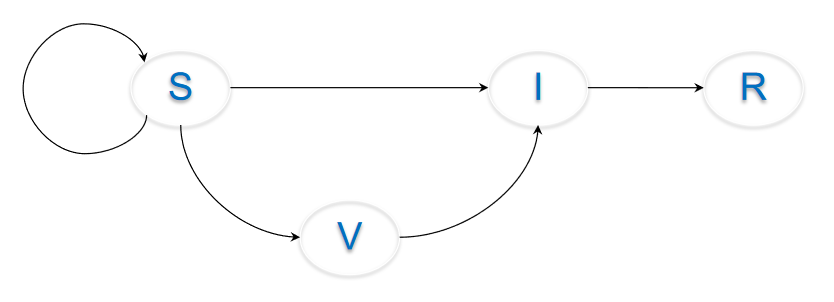
\includegraphics[width=0.5\linewidth]{img/SIRV.png}
    \caption{Susceptible, Vaccinated, Infected, Recovered model}
    \label{fig:sirv}
\end{figure}

\section{Kermack-McKendrick Epidemic Model}
The most basic epidemiological model was formulated by was first proposed 
by Kermack and McKendrick in 1927; this is a compartments model with 3 
classes:
\begin{itemize}
    \item $S(t)$ is the class of individuals who are healthy but can 
        contract the disease: these are called \textbf{susceptible} individuals;
    \item $I(t)$ is he class of individuals who have contracted the 
        disease and are now sick with it, called \textbf{infected} individuals;
    \item $R(t)$ is the class of individuals who have recovered and 
        cannot contract the disease again are called \textbf{removed/recovered} 
        individual;
\end{itemize}

\begin{figure}[!ht]
    \centering
    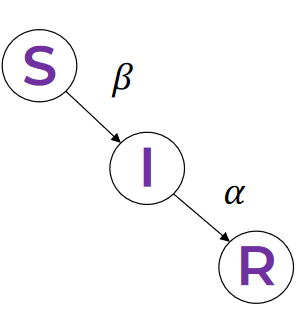
\includegraphics[width=0.25\textwidth]{img/SIR.png}
    \caption{Kermack-McKendrick Epidemic Model}
    \label{fig:SIR}
\end{figure}

This model is based on the following constraint:
\begin{enumerate}
    \item We suppose that each individual of a population could be 
        assigned into nonintersecting classes;
    \item It is assumed that infected individuals are also infectious;
    \item The number of individuals N in the population is fixed
        \begin{equation*}
            N = S(t) + I(t) + R(t)
        \end{equation*}
\end{enumerate}

Also, as we've seen in other simulation models we need to define the 
parameters. In this case, we have the following transition rates among 
the compartments.
\begin{itemize}
    \item $C$ is the probability for an individual to make a contact in 
        a unit of time (per capita contact rate);
    \item $C N$ is the total number of contacts per unit of time;
    \item $S/N$ is the probability that a contact is with a susceptible 
        individual;
    \item $C N (S/N)$ is number of contacts with susceptible individuals 
        of one infectious individual;
    \item $p$ is the probability that a contact with a susceptible 
        individual results in transmission;
    \item $p C S$ is number of susceptible individuals who become 
        infected per unit of time, per infectious;
    \item $p C S I$ is the number of individuals who become infected 
        per unit of time;
    \item Definition: $pC = \beta$ transmission rate constant;
\end{itemize}

Given that $\beta$ is defined as transmission rate constant, we can now 
state that:
\begin{equation}
    S'(t) = \beta I(t) S(i)
\end{equation}
Those individuals who recover or die leave the infected class at constant 
per capita probability recovery per unit of time $\alpha$, called the 
recovery rate. Hence, we have the following equations:
\begin{equation}
    I'(t) = \beta I(t)S(t) - \alpha I(t)
\end{equation}
\begin{equation}
    R'(t) = \alpha I(t)
\end{equation}

The SIR model have the following properties:
\begin{enumerate}
    \item The number of susceptible individuals is constantly declining;
    \item The number of recovered individuals is always increasing;
    \item The number of infected individuals increases if the following holds:
    \begin{equation*}
        \frac{\beta S(0)}{\alpha} > 1
    \end{equation*}
\end{enumerate}

Now, If we assume that there are no deaths or births in the population, we can solve
the differential equation as follow:
\begin{equation}
    \begin{array}{lc}
        S'(t) = & - \beta \frac{I(t)S(t)}{N} \\ 
        I'(t) = & \beta \frac{I(t)S(t)}{N} - \alpha I(t) \\
        R'(t) = & \alpha I(t)
    \end{array}
\end{equation}

Let's also consider to following ratio:
\begin{equation*}
    R_0 = \frac{\beta}{\alpha}
\end{equation*}
This number is called the \textbf{basic reproduction number} (or ratio). 
The number tells us what is the expected insurgence of “new” infections 
in a population where $S(0) = N - I(0), R(0) = 0$ and $I(0) = I_{initial}$

Whether $R_0 > 1$ or $R_0 < 1$ tells us how fast the disease is spreading.

The numbers $\beta$ and $\alpha$ can be thought of as rate constants of
yielding the expected times of infection (through a contact) and the time 
to recovery.
\begin{equation*}
    T_c = \frac{1}{\beta} \, \, \, T_r = \frac{1}{\alpha}
\end{equation*}

Solving the set of equations leads to the following relation:
\begin{equation}
    I(t) + S(t) - \frac{\alpha}{\beta} \ln (S(t)) = C
\end{equation}
Given initial conditions $I(0)$ and $S(0)$, the relation also holds 
for $t = 0$ and $t = \infty$.

From the rewriting of the equation for the number of infected people $
I(0)$, we can observe the following:
\begin{itemize}
    \item $R_0 S(0) > N \implies I'(0) > 1$
    \item $R_0 S(0) < N \implies I'(0) < 1$
\end{itemize}
Which tells us how important it is to establish the value of $R_0$.
\subsection{Variations on the SIR Model}
\begin{itemize}
    \item The Susceptible-Infected-Susceptible model (SIS) is used to 
        model diseases like the standard flu.
        \begin{figure}[!ht]
            \centering
            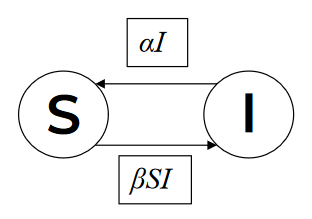
\includegraphics[width=0.25\linewidth]{img/SIS.png}
            \caption{Susceptible-Infected-Susceptible model}
            \label{fig:SIS}
        \end{figure}
    \item In the Susceptible-Infected-Removed-Deceased model (SIRD) a 
        new possible outcome is included: the possibility of death given an infection;
       \begin{figure}[!ht]
            \centering
            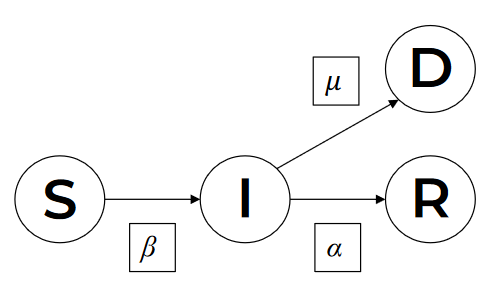
\includegraphics[width=0.25\linewidth]{img/SIRD.png}
            \caption{Susceptible-Infected-Removed-Deceased model}
            \label{fig:SIRD}
        \end{figure}
   \item The simplest one introduces a population of vaccinated (V) which           reduces the pool of susceptible people.
        \begin{figure}[!ht]
            \centering
            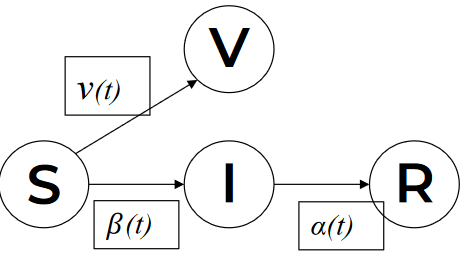
\includegraphics[width=0.25\linewidth]{img/SIRV1.png}
            \caption{Simplest one introduces a population of vaccinated}
            \label{fig:SIRV1}
        \end{figure}
\end{itemize}
\section{Network models}
Network models look at the spreading of an epidemics at an individual 
level and do not represent the populations as a compartment.

These methods represent either individuals or metapopulations, i.e., 
spatially separated groups of similar individuals, as a node of a complex 
network-

The contacts (the possible paths of transmission of the disease) are the 
edges of this network.
\chapter{Flux Balance Analysis}

The \textbf{Flux Balance Analysis} (FBA) is an analytical technique used to 
study biological systems from a metabolic perspective. The metabolism of a 
system is represented as a set of metabolic reactions, organized in a 
\textit{stoichiometric matrix} that describes these reactions. FBA allows us to 
study the flow of chemical substances through these reactions in the system.

\begin{definition}[\textbf{Metabolic pathway}]
    A \textbf{metabolic pathway} is defined as a sequence (or graph) of 
    metabolic reactions.
\end{definition}

When all metabolic pathways are considered and represented together, we obtain 
the metabolic network (or \textit{metabolome}) of the system, a section of which 
is illustrated in the figure \ref{fig:pathway}.

\begin{figure}[!ht]
    \centering
    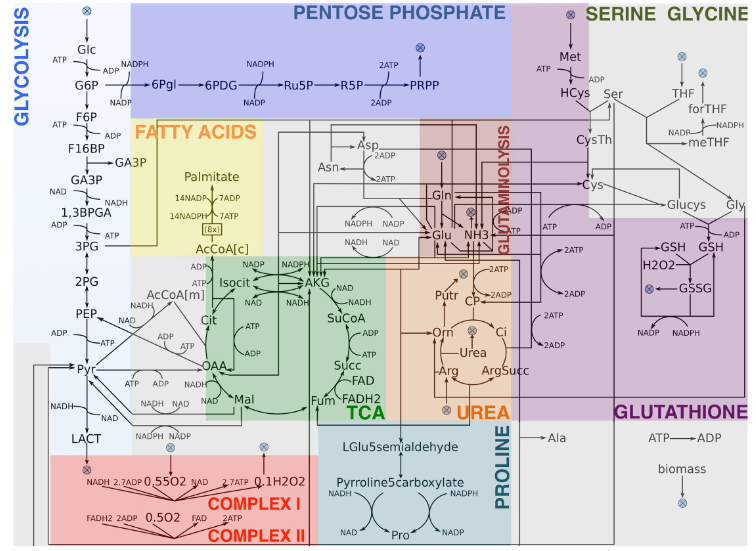
\includegraphics[width=0.5\linewidth]{img/pathway.png}
    \caption{A section of the overall metabolic network of a cell}
    \label{fig:pathway}
\end{figure}

An important aspect to consider when representing biological systems is the level 
of abstraction one wishes to adopt.

The study of cellular metabolism is crucial for understanding numerous diseases, including:
\begin{itemize}
    \item \textbf{cancer}: cancer cells utilize different metabolic pathways from 
        standard ones for energy production, and research focuses on both intracellular 
        metabolism (intra-tumor) and the interactions among cancer cells (inter-tumor);
    \item \textbf{diabetes}
    \item \textbf{obesity}
    \item \textbf{fatty liver disease}
    \item \textbf{Parkinson's disease}
    \item \textbf{Alzheimer's disease}
\end{itemize}

Additionally, metabolism research is fundamental for analyzing the effects of aging, as 
metabolic pathways change over time.

Another reason for studying metabolism is to explore its potential for metabolic engineering.

To identify the most active components within a system, it is useful to analyze metabolic flows. 
In practice:
\begin{itemize}
    \item it is possible to measure the \textbf{metabolome}, i.e., the concentration of metabolites 
        (end products or intermediates of metabolism) at a given time $t$;
    \item the \textbf{fluxome}, or metabolic flows over a time interval $\Delta t$, cannot be 
        directly measured.
\end{itemize}

\begin{definition}[\textbf{Flux}]
In this context, \textbf{flux} is defined as the difference between the rate of “forward” reactions 
and the rate of “reverse” reactions:
\begin{equation}
    \text{flux} = \text{rate}_{forward} - \text{rate}_{backward}
\end{equation}
\end{definition}

\section{Linear Programming}

Several modeling solutions exist to address the challenges of simulating biological systems:
\begin{itemize}
    \item \textbf{Static modeling}
    \item \textbf{Dynamic modeling}
    \item \textbf{Steady-state modeling}: an intermediate approach assuming the system is at 
        equilibrium, allowing simpler analysis.
\end{itemize}

In this context, linear programming is also employed, using:
\begin{itemize}
    \item The \textbf{stoichiometric matrix} $S$, where columns represent reactions and rows 
        represent metabolites;
    \item The \textbf{steady-state condition} expressed as $S \cdot v = 0$;
    \item The \textbf{flux constraints}:
        \begin{equation*}
            v_{min} < v < v_{max}
        \end{equation*}
        which describe different types of flux:
        \begin{itemize}
            \item \textbf{Input fluxes}, regulated by constraints on nutrients;
            \item \textbf{Internal fluxes}, regulated by thermodynamic and reaction 
                rate constraints;
            \item \textbf{Secretion fluxes}, to represent metabolic accumulation, modeling 
                growth and its constraints.
        \end{itemize}
\end{itemize}

Through linear programming, it is possible to calculate the \textbf{area of possible phenotypes}, 
defined by these constraints.

Exchange reactions are characterized by two parameters for reaction $R$, denoted as $R \Longleftrightarrow$:
\begin{itemize}
    \item \textbf{Uptake}: removal from the extracellular environment, or negative flux, 
        ranging from $-\infty$ to $0$;
    \item \textbf{Secretion}: introduction into the extracellular environment, or positive flux, 
        ranging from $0$ to $+\infty$.
\end{itemize}

The process of constraint-based modeling and Flux Balance Analysis (FBA) is as follows:
\begin{itemize}
    \item \textbf{Genome-scale metabolic reconstruction}: analyzing reactions and understanding the 
        pathways of the system;
    \item \textbf{Mathematical representation of metabolic reactions and constraints}, using a 
        stoichiometric matrix $S$, with additional columns for the variables of interest. This matrix is 
        multiplied by the vector 
        \begin{equation*}
            v = \{v_1, \dots, v_n, v_1', \dots, v_m'\}   
        \end{equation*}
        representing reaction flows, yielding $S \cdot v = 0$, a homogeneous linear system in 
        steady-state;
    \item \textbf{Mass balance}: defines a system of linear equations, $S \cdot v = 0$, which 
        represent the constraints of the system to be solved with linear programming;
    \item \textbf{Definition of an objective function} to optimize, of the form:
        \begin{equation}
            z = \sum_i c_i \cdot v_i
        \end{equation}
        where $c_i$ are the weights and $v_i$ are the target coefficients. The function $z$ is used 
        to predict values of interest;
    \item \textbf{Calculation of the optimal flux} that maximizes $z$ through linear programming.
\end{itemize}

Thus, linear programming is used with FBA to ensure flux feasibility, optimize a linear combination 
of the system’s products, and manage boundary conditions.

Naturally, this approach can become computationally complex. The well-known simplex algorithm is 
typically used, which is effective but may exhibit exponential complexity in certain cases.

Usually, using linear programming methods you get an optimal solution, this aspect can be
sometimes limiting. The problem to be faced is essentially that of ranking/choosing the 
different metabolic "states" which emerge in an analysis, when changing, for example, 
parameters or objective function. This kind of talk becomes interesting talking about 
\textbf{metabolic rewiring} (metabolic re-wiring) in the field of cancer.

FBA can be used in many ways, with various applications and extensions. These problems vary 
with the change in weights and objective function, some of them being partly solvable
numerically. All these aspects need to be studied and deepened from time to time.

From the point of view of linear programming, there are several categories of resolvers for 
the continuous case, but we can include them in two macro-categories:
\begin{enumerate}
    \item Solvers based on the simplex algorithm: they work well in most cases even if you 
        have "pathological" cases that make the problem exponential over time; 
    \item Solvers based on internal point methods: unlike solvers based on the simplex
        algorithm, you are guaranteed to find a solution in polynomial time. Unfortunately,
        these methods are difficult to implement.
\end{enumerate}
Besides the continuous case, we also have one in which we introduce integer constraints, 
with variables that belong only to N, thus having the whole linear programming. You can 
also have mixed problem solvers, both continuous and discrete, and these are quite complex 
and sophisticated.
\section{Exploring Fluxes}
During the analysis process we are interested in studying flows. The first step is to 
understand which of all the fluxes we can study are most interesting for us. To do this, 
we start with a complete model (\textbf{Genome Wide Reaction Models}), which is very complex
for the study because it is biologically very realistic and complete, and we proceed to build
a \textbf{Core reaction model}. These models are obtained by simplifying complex models and
grouping reactions, thus obtaining models ready for simulation. In practice, you take a
piece of pathway and ignore the intermediate steps, compacting the representation, simplifying
equations and computational complexity.
\section{Enhanched Growth Model}
We now study the \textbf{ENGRO} model shown in Figure \ref{fig:engro}, which represents the
core model used to represent the growth of a cell. This model has led to the observation that 
cancer cells and many glass-grown cells have a glucose fermentation process, even when there 
is enough oxygen to breathe properly. In other words, instead of fully breathing in the 
presence of an adequate level of oxygen, cancer cells ferment. Currently, it is thought that 
cancer cells ferment glucose while maintaining the same level of respiration that was present 
before the carcinogenesis process, and therefore the Warburg effect would be defined as the 
observation that cancer cells show glycolysis with lactate secretion and mitochondrial 
respiration in the presence of oxygen. 

\begin{figure}[!ht]
    \centering
    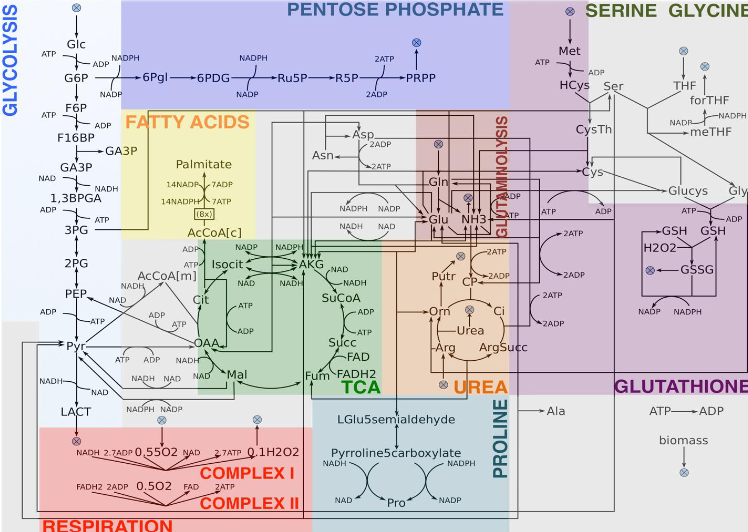
\includegraphics[width=0.5\linewidth]{img/ENGRO.png}
    \caption{Modello ENGRO}
    \label{fig:engro}
\end{figure}

To study this system, we did not limit ourselves to a single objective function of linear 
programming, but studied several, having in fact a meta-programming problem. The entire space
of the FBA solutions is then studied, as well as how a model can be \textbf{perturb} and again used to analyse the perturbation.

The first step is to analyse the results obtained with FBA. For example, if one wants to look
for the optimal value of the growth rate in function of the availability of nutrients entering 
the system one can start by noting that when the amount of glucose drops a greater quantity of 
oxygen is required and vice versa.

An initial study that can be carried out with the ENGRO model is therefore to place certain 
constraints on substances entering the system, or to place constraints on certain flows. This 
is done to study, in the light of a certain objective function, the optimal distribution of 
flows. In particular, we will see which of these are up-regulated and which down-regulated.
Obviously, the optimal solutions can be different, it is therefore a good rule to explore the 
whole space of acceptable solutions, varying the various weights of the objective function 
etc$\dots$, also making certain reactions enable/disable from time to time.

Consider, for example, the following conditions on the set of solutions and on a number $j$ of 
interactions:
\begin{equation}
    \begin{split}
        \sum_{i \in NZ_{j - 1}} y_i \geq 1 \\
        \sum_{i \in NZ_j} w_i \leq |NZ_k|-1 \, \, \, \text{for} \,\,\,k = 1, 2, \dots j - 1\\
        y_1 + w_i \leq 1, \,\, \forall i \\ \alpha \cdot w_i \leq v_i \leq \beta \cdot w_i \, \, \forall i
    \end{split}
\end{equation}
At each iteration $j$, at least one of the non-zero flows from the previous solution, namely 
$NZ_{j - 1}$, shall be set to zero, where the binary variable $y_i$ is 1 if that fluxe is 
selected to be removed from base at iteration $j$. The binary variable $w_i$ is then forced to 
zero if $y_i$ is one, and the upper and lower bounds for that particular stream are then bound 
to zero.

The equations ensure that alternative bases are not revisited by removing at least one non-
zero variable found in previous iterations. This is therefore a recursive algorithm for the 
calculation of alternative optimals using mixed integer linear programming (MILP) and allows 
us to enumerate the various alternative solutions.

Another interesting thing to study is how the phenotype changes as certain disturbances in the
system vary. To do this, we then start with a wild-type phenotype and apply various changes to 
it in order to obtain a modified phenotype. The following disturbances can be applied to 
obtain this result: (\textit{i}) nutrient disturbances, (\textit{ii}) gene deletion.
In addition, other tests may be performed less frequently, such as: (\textit{i}) deletion of
reactions, (\textit{ii}) thermal shock.

From the most modelling/mathematical point of view, there are various ways of studying the 
disturbance of the system. A first approach is to use simply the FBA, simulating metabolic 
responses, for example by studying knockouts (which could be multiple in the system under 
analysis) and nutrient variation. Let us take an example where, in the wild-type case, we want 
to maximize growth. There is thus a certain objective function with certain constraints, such 
as:
\begin{equation}
  \begin{array}{rrclcl}
    \displaystyle \max & f_{growth} \\
    \textrm{s.t.} & b_L & \leq & f & \leq b_{U} \\
                       & Sf & = & [0] \\
  \end{array}
\end{equation}
We can add constraints to obtain:
\begin{equation}
  \begin{array}{rrclcl}
    \displaystyle \max & f_{growth} \\
    \textrm{s.t.} & b_L & \leq & f & \leq b_{U} \\
                    & Sf & = & [0] \\
                    & b_L & \leq & f_{mut} & \leq b_{U} \\
  \end{array}
\end{equation}

The added constraints can be used to represent one of the above listed disturbances.

However, there are still some limitations:
\begin{itemize}
    \item The mutation may not grow optimally if natural selection has not had a chance to act on the new genetic background;
    \item has "only" found an excellent alternative, having however, from the point of view of linear programming, solutions that are located on the vertices;
\end{itemize}
This procedure is however usually automated, perhaps using a list of genes to be activated/
deactivated, keeping track of each change and the variation in results obtained through it.

Overcoming the classical approach, the first step is to introduce a particular biological 
hypothesis, called the Minimization of Metabolic Adjustment (MOMA) hypothesis, which assumes 
that a mutation will tend to approximate when it has the wild-type as much as possible. More 
formally a MOMA flow vector with minimum euclidean distance from a single optimal wild-type 
entity is found, subject to the constraints of the mutation. There is thus a certain objective 
function with certain constraints, such as:
\begin{equation}
  \begin{array}{rrclcl}
    \displaystyle \max & f_{growth} \\
    \textrm{s.t.} & b_L & \leq & f & \leq b_{U} \\
                    & Sf & = & [0] \\
  \end{array}
\end{equation}
using MOMA:
\begin{equation}
  \begin{array}{rrclcl}
    \displaystyle \min & |m -f_{opt}| \\
    \textrm{s.t.} & b_L & \leq & f & \leq b_U \\
                    & S_m & = & [0] \\
                    & b_L \leq f_{mut} \leq b_U
  \end{array}
\end{equation}

Thus obtaining not an excellent on a summit but the closest solution, under the MOMA hypothesis. Obviously, there are limitations here too:
\begin{itemize}
    \item the MOMA hypothesis will push the metabolism in the mutant towards the arbitrary distribution of single optimal flow obtained with the FBA but there are still alternative solutions that maximize growth and other sub-optimal solutions
    \item growth is not assured in the mutations
\end{itemize}

Another approach is the more probabilistic one, based on a random sampling of the various 
parameters of linear programming. There are therefore two types of sampling approach:
\begin{itemize}
    \item \textbf{Hit-and-Run} (HR), where you have uniform sampling within the region of the
        allowed solutions, that is a valid initial point is moved repeatedly into space
        according to probabilistic rules. An objective function of the type is obtained by
        having a random pair of reactions:
        \begin{equation*}
            F = w_i \cdot f_i + w_j \cdot f_j
        \end{equation*}
    \item \textbf{Convex Basis} (CB) where the simplex algorithm is used with a random set of
        objective functions to be maximized. Maximising each of these objective functions will
        give a corner in the space of solutions.
\end{itemize}
Obviously the number of combinations that can be obtained with sampling can be really huge so
it must be carried out "under control".

Another interesting element is the so-called ENGRO \textbf{Z-score}. Such value other does not
measure the difference between mutation and wild-type entity, by measuring on wild-type means
and standard deviation:
\begin{equation}
    Z = \frac{\overline{X}_1 - \overline{X}_2}{\sqrt{\frac{\sigma^2_1}{n} + \frac{\sigma^2_2}{n}}}
\end{equation}
Having therefore a high value for Z corresponds to a high difference between the wild-type 
entity and the mutation.
\section{Guiding the Search}
The current study of FBA-based methods has several limitations, although some extensions have 
been created to overcome them. Among the various limitations we have:
\begin{itemize}
    \item Is based on the assumption of steady-state, leading to difficulties in studying the
        dynamics of the system
    \item does not provide any information on the concentrations of metabolites
    \item Requires limited choice of objective function
    \item has a limit in predicting the net behaviour, or the sum of flows, of possibly 
        heterogeneous cells within a population.
\end{itemize} 

It was also asked whether the metabolism works only to maximise the growth rate. There is
evidence, studied in the laboratory, that the deletion of some metabolic genes cause an 
increase in growth rates and biomass yield compared to the wild-type entity. The selective 
pressure to increase growth rate must be balanced by other demands on metabolism, such as 
cellular maintenance or sensory apparatus, reducing growth rate in favor of overall fitness. 
Also, limitations of evolutionary time and genetic variability may mean that metabolism is not 
optimal for any target, so we cannot necessarily exclude from consideration the many flow 
configurations that support, for example, $90\%$  (but also percentages) of maximum growth.
These support configurations are useful when deciding linear programming constraints.

The key point of the speech is that perhaps with an optimal solution from the point of view 
of the growth rate it leads to maximize biomass while with a sub-optimal solution, always side 
growth rate, you get not only an acceptable biomass but maybe also, For example, the 
production of other components, perhaps biofuels.
\section{Metabolic Pathways Rewiring}
We can see cancer as a "stochastic disease", resulting from a series of mutations affecting the 
cells of our body and involving the selection of a phenotype useful solely for its own purposes. 
Cancer cells are therefore, roughly speaking, part of normal cell sets that have accumulated a 
random set of mutations and epigenetic modifications. It is therefore that the cellular evolution 
has been in these cases somewhat modified and then we can study the normal functioning of metabolism, 
this sort of "metabolic wiring" ("metabolic connection") of those sets that have generic properties 
which statistically correspond to the real cell properties. 

In more mathematical terms we recognize the area of feasibility through linear programming. Outside of 
this area you have the impossible phenotypes while inside you have all the phenotypes possible, where 
various subsets with similar properties can be identified. The metabolism is therefore assumed to be 
similar between normal and carcinogenic cells, but if does a different study through the FBA.

To explore the space of possible "links" we proceed by random sampling of weights, changing objective 
function each time, and also sampling reactions, aiming finally to maximize the sum of the flows through 
certain reactions. The flow distributions obtained may be an efficient representation of a randomly 
mutated cell population. 

After making various analyses through the FBA, sets of different metabolic responses to disturbances 
are created and a sort of binary tree is created, which is divided according to the success rates of 
certain actions. From this tree, different information can be obtained on the system, since the different 
branches allow us to distinguish normal behaviour from carcinogenic behaviour.
\chapter{Reconstructing Cancer Progression Models}
In Figure \ref{fig:CRC}, there is an example of the evolution of Colon Rectal Cancer (CRC). 
The progression modes are multiple and the study of these is central in the discourse 
of so-called personalized medicine. Always talking about CRC The concept of staging 
must also be introduced. The progression of the tumor occurs in several steps, in 
detail of CRC are identified tendentially 4, each with its sub-stages, which lead from 
the initial state to the now uncontrolled development and metastasis of the tumor also 
in other organs.

\begin{figure}[!ht]
    \centering
    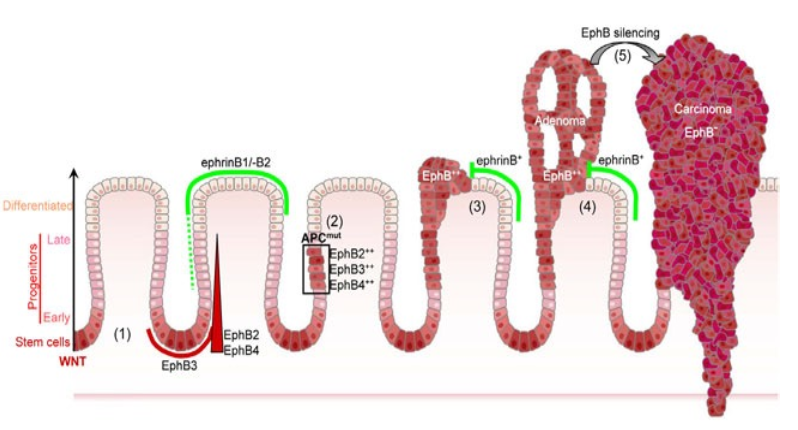
\includegraphics[width=0.5\linewidth]{img/CancerProgression/CRC.png}
    \caption{CRC Standard Progression}
    \label{fig:CRC}
\end{figure}

In this context, the study of images is also interesting, both through a committee of doctors 
who determine the extent of tumor progression, and, more computationally, using machine learning 
models and artificial intelligence techniques for image analysis. A good hypothesis, on most
types of cancer, is that the tumour progresses through \textbf{stages} by accumulating 
alterations affecting gene function and interactions. The following conclusions can be drawn:
\begin{itemize}
    \item The malfunction of individual genes cannot cause cancer. It has been understood that 
        a tumour is the result of multiple malfunctions of different genes;
    \item Cancer develops through multiple evolutionary pathways, so it is a problem to 
        where it actually develops;
    \item The alterations can be categorized in various ways, but among the main ones are:
        \begin{itemize}
            \item \textbf{Somatic mutations}: is a mutation at the DNA level of any cell in 
                the body. If the affected cell is still able to divide, the mutation is 
                transmitted to all cells resulting from it by mitosis. In this case the 
                organism will consist of a population of normal cells and one of mutated cells;
            \item \textbf{Copy number variation} (CNV): the phenomenon where sections of the
                genome are repeated and the number of replications in the genome varies from
                individual to individual. The variation of the number of copies is a type of
                structural variation: specifically, it is a type of duplication or deletion 
                event that affects a considerable number of base pairs, involving for example over-expression of certain proteins;
        \end{itemize}
        These, and many other events are due to countless factors, so the causes of cancer 
        progression can be really multiple
\end{itemize}

So, this whole modelling study is essential for drug development and for therapeutic decisions,
for example, for the same type of cancer, patients in different stages/stages of different 
progressions respond differently to different treatments.

Cancer cells are like other cells and can therefore be studied as individual replicators. 
The purpose is the same as normal cells, that is they have the objective to reproduce must
therefore:
\begin{enumerate}
    \item \textbf{Grow}: through energy consumption and nutrients;
    \item \textbf{Live long and prosper}, and therefore limit/avoid apoptosis;
    \item \textbf{Move}: in the case of cancer cells this is done by metastasis.
\end{enumerate}
A cancer cell is therefore essentially a cell which has exchanged a series of behaviors, 
dictated by its genetic make-up, for others more "successful" in its microenvironment,
unfortunately the concept of "successful" for the cell is a problem for the organism. 

By succeeding in replicating, these cells give rise to a new (\textbf{sub})\textbf{clonal}
population that continues to expand, thus generating neoplastic growth, or the abnormal 
growth of cells that leads to cancer.

Over the years, external causes of cancer have also been discovered. This adds further 
complexity to the studies.

It is now necessary to understand what are the \textbf{hallmarks} of cancer, the so-called 
cancer hallmarks. Cancer hallmarks represent a "new" mode of operation, giving cancer cells 
forms of selective advantage. These are described as follows:
\begin{itemize}
    \item \textbf{Self-sufficiency in growth signals}: remembering that at the cellular level
        signals are received by cells via proteins;
    \item \textbf{Insensitivity to anti-growth signals} that seek to limit uncontrolled tumor
        growth;
    \item \textbf{Avoid programmed cell death}: avoiding apoptosis reported by p53;
    \item \textbf{Unlimited replicative potential};
    \item \textbf{Making angiogenesis}: the process that leads to the formation of new blood
        vessels from other pre-existing vessels, sustained. This tells the circulatory system to 
        create blood vessels near the tumor so that it can better supply growth substances;
    \item \textbf{Tissue invasion} and \textbf{Metastasis};
    \item \textbf{Deregulate metabolism} (and that's what is being studied with FBA)
    \item \textbf{Evading the immune system}, which reacts not only with apoptosis but also 
        with many other operations;
    \item \textbf{Lead to genome instability}.
\end{itemize}
All these points are extreme behaviors that a normal cell would have anyway to grow, move 
and live long.

When it comes to cancer progression, we can draw a parallel with Darwin’s study of evolution. 
We can see how it starts with a certain normal cell that in a certain micro-environment at a
certain moment of time divides, accumulating in the various micro-environments various mutations 
and creating the tumor situation. A clone arrives and survives when it is "better" than the 
normal cells and other clones, eventually ending up with only clones.

The study of these problems is based on the data produced by sequencing and the creation of 
graphs such as that shown in Figure \ref{fig:CE}. 

\begin{figure}[!ht]
    \centering
    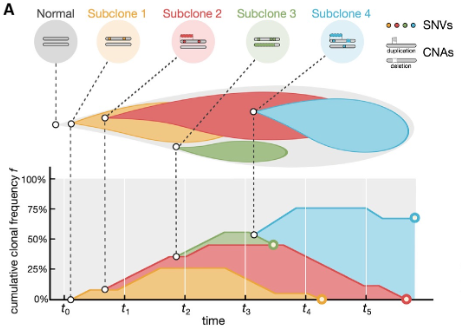
\includegraphics[width=0.5\linewidth]{img/CancerProgression/CE.png}
    \caption{Clonal Expansion}
    \label{fig:CE}
\end{figure}

Data is often problematic:
\begin{itemize}
    \item Missing data, for various technical reasons;
    \item Lack of useful time points. There are often very distant time points and with 
        uneven and increasing distances, mainly due to the method of experimentation used.
\end{itemize}

In general, these studies are useful to understand whether a particular cure is having the desired effect. For example, if we look at the Figure \ref{fig:Resistance}, we can see that 
some strains manage to survive the treatment. This can lead to a reappearance or the 
emergence of new mutations.

\begin{figure}[!ht]
    \centering
    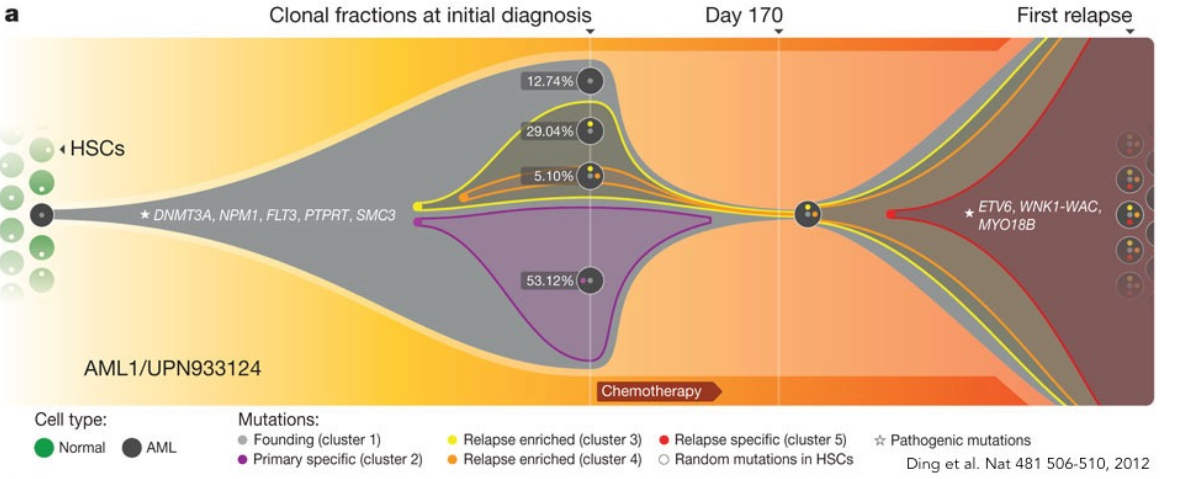
\includegraphics[width=0.5\linewidth]{img/CancerProgression/Resistance.png}
    \caption{Clonal Expansion and Resistance}
    \label{fig:Resistance}
\end{figure}

Another interesting aspect is the \textbf{Inter-Tumor} and \textbf{Intra-Tumor Heterogeneity} 
(ITH). The ITH is however a difficult subject to treat and study. Within a tumor in the same
patient there are variations, such as spatial and clonal heterogeneity, but there are also 
variations between the same tumor in different patients, thus having to make facets of 
heterogeneity.
\section{Cross Sectional Data}
A very important aspect in studying the evolution of cancer is to understand how data is collected 
and what it represents. In particular, there are two type of study:
\begin{enumerate}
    \item \textbf{ensemble-level}: Attempts to reconstruct a set of plausible precedence 
        relationships of events from patient data, which can be many. This is done from $n$ 
        independent cross-sectional data. We can imagine having a matrix with $n$ patient 
        genomes for the columns and $m$ "conductive events".
    \item \textbf{individual-level}: The attempt is to reconstruct a tumor cell population 
        from tissue samples using single-cell and phylogenetic techniques. In this case, we 
        start with $n$ samples of the same tumor, obtained from a biopsy, and sequenced by 
        bulk sequencing. The evolutionary tree is then obtained of a single tumor and study 
        the ancestral tumor and clones without generalizing selection, studying specifically 
        for the individual patient.
\end{enumerate}

We now want to go deeper into the ensemble-level, through cross-sectional data, as this type of 
data represents the majority of available cancer data. 

These data are collected through biopsies taken at the time of diagnosis. It is therefore a set 
of data that is collected only the first time and then you do not know what happens next. All 
these datasets are sorted so that results can be obtained on the tumour evolution. Inferring 
time information from such data is still an open challenge. 

We also know that these data are very noisy and often handled with machine learning techniques 
and neural networks. Another key aspect to consider is the missing data, which complicates matters 
further.

There are several databases that maintain and update information on cancer. The best known is 
\textbf{The Cancer Genome Atlas} (TCGA), which provides several portals to simplify access to data.
\subsection{Analysis}
We would like to answer the following questions:
\begin{enumerate}
    \item Can we reconstruct a progression model from cross-sectional data?
    \item What is actually contained in the datasets and what is actually contained in the 
        cross section, having changed a lot over the years?
    \item What kind of models can we rebuild?
\end{enumerate}

Let’s see how it is possible to reconstruct the progression models by using Direct 
Acyclic Graph (DAG), which encodes the accumulation of alterations and mutations. A useful 
library in this context is TRONCO, which contains various techniques and algorithms for the 
reconstruction of progression models.

In answering the first question, we can reconstruct a progression model from the creoss-sectional 
data. In addition, from these models, you can get tips on the correct therapies to use to treat 
a patient. The procedure for doing so is as follows:
\begin{itemize}
    \item • It starts from a \textit{Boolean matrix} where the columns are mutations and the rows 
        are tumors, indicating with 1 and 0 the presence or absence of a certain mutation in a certain tumor.
    \item A causal network is created where it is specified which mutation causes. Thus, a concept of
        "precedence" is obtained;
    \item The network then studies the mutual causality between mutations.
    \item The results are used to study pathway causality or phenotypes, or hallmarks, and therefore 
        have additional levels of abstraction from generic DAG.
\end{itemize}

As regards the second question, the public databases for cancer data must be used again. All these
databases address the problem of centralizing data and information, which until a few years ago 
were also quite expensive.

Obviously, in the field of cancer research, the most interesting information from databases, among 
the many available information, is that relating to mutations, which are usually inherited and 
persistent between successive generations of cancer cells. The most interesting mutations are usually 
those of somatic character, that is somatic mutations. In addition, it is more said that the probability
of occurrence of a given alteration is related to how functional it is to the development of the tumor,
having therefore that you have the mutations called driver and passenger, as well as different rates of 
tumor mutation. Of course, mutations can also be of various types:
\begin{itemize}
    \item The so-called single nucleotide variant (SNP), or single base mutations;
    \item Loss of heterozygosity, with loss of genomic regions, loss of smaller portions, 
        copy-number mutations etc$\dots$
    \item Whole deletions that are terminal or internal to the sequence
    \item Duplications of parts of sequences that can lead to tandem, where the duplications are next 
        to each other, or duplications where the duplicate portions are separated from each other by 
        another portion of the genome;
    \item Amplifications of genomic portions of intra-chromosomal and inter-chromosomal types; 
    \item Duplication of the entire genome.
\end{itemize}

To answer the third question we can use various studies which have defined the following models:
\begin{itemize}
    \item \textbf{Tree models}: these models are based on correlations;
    \item \textbf{Joint models}: mainly based on Bayesian models;
    \item \textbf{DAG models}: which are a generalization of the two previous models.
\end{itemize}

Let’s now look at some techniques developed in the DCB bicocca research laboratory:
\begin{itemize}
    \item \textbf{CAncer PRogression Extraction with Single Edges} (CAPRESE), for tree modelling.
    \item \textbf{CAncer PRogression Inference} (CAPRI), an extension of CAPRESE to work through 
        DAG models.
    \item These algorithms, plus other supporting features such as access to cBIO and TCGA, have 
        been collected in the R language library called \textbf{Translational ONCOlogy} (TRONCO).
\end{itemize}

Suppose you want to model a tumour progression in which two mutations occur, one called EGFR and 
then one called CDK. Two important assumptions must be made in order to proceed with the modelling:
\begin{enumerate}
    \item \textbf{Persistence assumption}: acquired mutations do not disappear. The EGFR mutation
        therefore gives a selective advantage, and then the clonal expansion is carried out. This 
        also increases the likelihood of acquiring a CDK mutation. When both mutations are present, 
        one species is selectively even more favoured;
    \item \textbf{Event selection assumption}: that is, events relevant for progression must be chosen 
        in advance. In practice, it is already known that a model with the EGFR and CDK mutations must 
        be studied. Limiting to a few combinations of events makes the reconstruction computationally 
        feasible, thus not using the entire multitude of data from oncology studies. It is then done a 
        sort of supervised study to find the driver mutations.
\end{enumerate}

Another key aspect in this study is that each patient has a different history of cancer evolution 
and progression. The actual input to the progression reconstruction algorithm can be thought of as 
a set of possible trajectories, that is, sequences of genomic alterations that accumulate in 
different ways. You must then proceed with counting and assigning the correct probabilities to each 
single occurrence of an event.

Over the years, various models have been developed to reconstruct tree or DAG models and all algorithms
need a measure to decide whether and how to include an arc in the reconstruction. In the above 
mentioned algorithms, it was chosen to use the theory of probabilistic causality.

Another key aspect in this study is that each patient has a different history of cancer evolution and
progression. The actual input to the progression reconstruction algorithm can be thought of as a set of 
possible trajectories, that is, sequences of genomic alterations that accumulate in different ways. You 
must then proceed with counting and assigning the correct probabilities to each single occurrence of an 
event.

Over the years, various models have been developed to reconstruct tree or DAG models and all algorithms 
need a measure to decide whether and how to include an arc in the reconstruction. In the above mentioned 
algorithms, it was chosen to use the theory of probabilistic causality.

The core of this theory is very simple. Two events $c$ and $e$, occurring respectively at time $t_c$ 
and $t_e$, are given with:
\begin{equation*}
    0 < P(c) \,\, \land \,\, P(e) < 1    
\end{equation*}
There is a \textit{prima facie} cause for $e$ if two properties are respected:
\begin{enumerate}
    \item The time priority property, that is:
        \begin{equation*}
            t_c < t_e
        \end{equation*}
        this ensures a time order between events.
    \item The property of probability growth, which tells us that the probability that the event $e$
        happens having happened to $c$ event is greater than that in which you do not have event $c$:
        \begin{equation*}
            P(e| \lnot c) < P(e|c)
        \end{equation*}
\end{enumerate}
These two properties, necessary but not sufficient, guarantee the directionality of the model.

In addition to the Suppes theory, both measurements and theoretical analyses are reinterpreted in
biologically plausible terms, possibly also by redefining selective advantage relationships. 

Let us then go into more detail on the basis for reconstructing the progression model. The already
anticipated prima facie cases can be of two types:
\begin{itemize}
    \item Authentic/genuine, the "correct ones";
    \item Spurious, "wrong" ones.
\end{itemize}
Therefore, the two conditions are only sufficient and not necessary. Also, speaking of cross-sectional
data, the time priority between events is not known, so the problem of reconstruction becomes more 
difficult. 

The problem becomes how to establish whether a given arc between two events corresponds or not to a 
false cause, and therefore should not be considered, since the interpretation of an arc will be that of 
a selective advantage relationship between genetic events.

In addition, a further complication is given by the fact that nothing ensures that we speak only of two
events but we can have complex combinations of causality between events. For this reason, in the CAPRI 
algorithm these situations are managed by means of boolean formulas, like the conjunctive formulas of 
the type used in the Bayesian conjunctive networks. 

The following are distinguished:
\begin{itemize}
    \item \textbf{Singleton}: where one mutation occurs before another and there is a causal relationship;
    \item \textbf{co-occurrence}: where more than one mutation occurs before another and there is a 
        causal relationship. Obviously, in this case the complexity increases.
\end{itemize}

In the CAPRI algorithm there is also a final condition, that is the condition for the selection
advantageous through patterns:
\begin{equation*}
    c e \Longleftrightarrow P(c) > P(e) \,\, \land P(e | c) < P(e| \lnot c)
\end{equation*}

We then start with a causal model with selective advantages, make observations on imperfect regularities
and frequency studies. More specifically, the inference of results is then obtained by statistical
techniques such as:
\begin{itemize}
    \item \textbf{boostrap}: a statistical technique of resampling with resampling to approximate the
        sample distribution of a statistic. It therefore allows you to approximate the mean and variance
        of an estimator, construct confidence intervals and calculate test p-values when the distribution
        of interest is not known;
    \item \textbf{p-value} and other tests.
\end{itemize}

Causal relationships between mutations are thus obtained, possibly also with the co-occurring effect 
of several mutations causing a third mutation.

For complex patterns it has been studied experimentally as the CAPRI algorithm which is able to understand
the causality between various mutations and represent them by Boolean formulas. The complexity of the 
model then leads back to the complexity of such formulas.

Boolean formulas are of the conjunctive normal form (CNF), or a conjunction of clauses, where clauses are
a disjunction of literal ones.

In order to limit complexity we must therefore highlight the most significant authentic relationships. 
The CAPRI algorithm is a combination of six steps which are responsible for producing a set of 
selectivity relationships and then cleaning up the generated model:
\begin{enumerate}
    \item Input data management;
    \item Pre-processing with addition of information, called lifting, to the raw model obtained from the
        data. We have a set $G$ of $n$ events from $m$ cross sectional samples, having therefore a Boolean 
        matrix $n \times m$. In this one we assume a set of hypotheses:
        \begin{equation*}
            \Phi = \{\phi_i \rhd e_i | 1 \leq i \leq k\}, \text{ con } k + n \ll m
        \end{equation*}
        Each individual $\phi \rhd e_i$ is used to increment the matrix into input by obtaining a 
        $D(\Phi)$ matrix that encodes optional selectivity relations as events.
    \item DAG node selection;
    \item DAG edge selection;
    \item There is then a phase of labeling the arcs. At this stage the coded selectivity relations are CNF 
        formulas, so they can be treated in a composite way by separately checking each conjunction. The algorithm
        includes in the construction arcs between two events $c$ and $e$ if and only if:
        \begin{equation*}
            P(c) - P(e) > 0 \,\,\land P(e | c) - P(e | \lnot c) > 0
        \end{equation*}
        and this is the main condition. Note that the probabilities are estimated from the data directly, through 
        a first step of boostrap. The reconstructed DAG contains all the correct selectivity relationships but also 
        several spurious ones, which are not yet eliminated.
        
        Each arc is labeled with a probability which is essentially the probability of observing a certain mutational 
        profile in a sample.
    \item Finally a likelihood fit phase. Recalling that the Suppes assumptions are only necessary to "filter" spurious
        relationships, ie false positives that have been included in the previous steps, we calculate a fit of maximum
        likelihood that includes a regularization term, The term may be chosen and calculated differently.

        Finally, a bootstrap pass is used to deduce the confidence intervals for each selectivity relation inferred.
\end{enumerate}

The CAPRI algorithm is correct and complete, since only true selectivity relationships deductible from the data are
reported.

It should always be remembered that the precedence relations which the algorithm deduces do not explain the 
mechanistic biochemical causes of a progression model, In fact, the algorithm only makes a statement that 
observing a given set of mutations increases the probability of seeing one later.
\end{document}